\documentclass[12pt,a4paper,openright,twoside]{book}
\usepackage[utf8]{inputenc}
\usepackage{disi-thesis}
\usepackage{code-lstlistings}
\usepackage{notes}
\usepackage{shortcuts}
\usepackage{acronym}
\usepackage{hyperref}
\usepackage{biblatex}
\usepackage{changepage}
\usepackage{enumitem}
\usepackage{caption}
\usepackage{subcaption}
\addbibresource{bibliography.bib}

\school{\unibo}
\programme{Corso di Laurea in Ingegneria e Scienze Informatiche}
\title{Sviluppo di un sistema di visione artificiale per la rilevazione e localizzazione di marker ArUco in un contesto di aggregate computing}
\author{Bacchini Lorenzo}
\date{\today}
\subject{Programmazione ad oggetti}
\supervisor{Prof. Mirko Viroli}
\cosupervisor{Dott. Gianluca Aguzzi}
\session{III}
\academicyear{2023-2024}

\mainlinespacing{1.241} % line spacing in mainmatter, comment to default (1)

\begin{document}

\frontmatter\frontispiece

\begin{abstract}
Il paradigma dell'aggregate computing rappresenta un nuovo approccio alla programmazione distribuita, focalizzando l'attenzione sulla definizione di comportamenti globali che vengono poi interpretati dai singoli dispositivi. L'elaborazione finale non avviene dunque su un sistema esterno, ma sono i dispositivi stessi a comunicare tra loro per prendere decisioni basate sul raggiungimento di un fine comune.

In questo contesto si inserisce un progetto sviluppato dai ricercatori dell'università di Bologna, volto a gestire uno sciame di robot o droni secondo algoritmi distribuiti e comportamenti auto-organizzativi.
Generalmente in sistemi come quello sopra citato la localizzazione dei robot avviene grazie a tecnologie di posizionamento satellitari, nel caso in questione però è necessaria l'implementazione di una soluzione in grado di operare anche in ambito indoor, mantenendo costi contenuti e un'infrastruttura quanto più semplice possibile.

Al giorno d'oggi la visione artificiale trova applicazioni in una grande vastità di settori, dalla ricerca all'ambito industriale, con lo scopo di replicare la vista umana. L'uso di tali tecniche è ormai supportato da numerose librerie software ed è largamente diffuso, pertanto si è scelto di analizzare tale approccio al problema posto, sviluppando in questa tesi un sistema di posizionamento basato sul riconoscimento di marker ArUco, ottenuto grazie all'utilizzo della libreria di visione artificiale OpenCV.

I risultati conseguiti in questa dissertazione dimostrano la precisione dei sistemi di localizzazione basati su processi di visione artificiale, analizzando però i limiti di questa tecnologia in termini di condizioni ambientali e contesti di utilizzo.
\end{abstract}

\begin{dedication} % this is optional
Alla mia famiglia
\end{dedication}

%----------------------------------------------------------------------------------------
\tableofcontents
\listoffigures
\lstlistoflistings
%----------------------------------------------------------------------------------------

\mainmatter

%----------------------------------------------------------------------------------------
\chapter{Introduzione}
Il mondo del lavoro e la vita di tutti i giorni stanno notevolmente cambiando grazie all'avvento di nuove tecnologie, che in maniera più o meno evidente stanno invadendo la nostra quotidianità, ne sono la prova la moltitudine di dispositivi con la quale interagiamo costantemente come smartphone, smartwatch, smartbands, smartglasses ecc.
Anche in ambito industriale stiamo assistendo alla formazione di quella che viene comunemente chiamata ``Industria 4.0", la quale promette di portare gli attuali sistemi informatici e di automazione ad un livello successivo basato sulla collaborazione e comunicazione degli stessi.
Un tema emergente nell'ambito di sistemi distribuiti collaborativi è rappresentato dal paradigma dell'aggregate computing.

Il paradigma dell'aggregate computing~\cite{VIROLI2019100486} si differenzia dalla programmazione distribuita in quanto maggiore enfasi è posta sulla definizione di un obiettivo globale che il sistema deve raggiungere, piuttosto che sulle regole e sui singoli compiti che ogni nodo deve portare a termine, elevando così il livello di astrazione.

A partire da questo nuovo paradigma i ricercatori dell'università di Bologna hanno sviluppato un software capace di controllare una serie di robot/droni. Sulla base di concetti derivati dalla robotica degli sciami, esso consente ai dispositivi di auto-organizzarsi e conoscere lo stato generale del sistema, scambiando informazioni con i propri vicini.
Un aspetto fondamentale del progetto sopracitato è dato dalla possibilità di determinare in ogni istante la posizione dei robot, operazione triviale in ambito outdoor, dove per localizzare i dispositivi è sufficiente un segnale di posizionamento satellitare per ottenere dei risultati precisi, dovendo però nel nostro caso utilizzare tale sistema all'interno di edifici, dove un segnale GPS non sarebbe in grado di fornire una precisione sufficiente rende indispensabile esplorare approcci alternativi.

La visione artificiale rappresenta una soluzione economica e poco complessa a tecnologie ben più articolate e soprattutto costose in materia di sistemi di posizionamento indoor. L'obiettivo di questa tesi è quello di approfondire l'utilizzo di tecniche di visione artificiale con l'aiuto di librerie software come OpenCV, con il fine ultimo di ottenere un applicativo in grado di rilevare e localizzare i dispositivi in una determinata scena, così da fornire ai ricercatori dell'università di Bologna un sistema finito da poter integrare all'interno del loro progetto per renderlo utilizzabile anche in contesti indoor.

\begin{center}
	Di seguito viene fornito il link al sistema sviluppato \url{https://doi.org/10.5281/zenodo.14039135}
\end{center}
\paragraph{Struttura della tesi}

Nel primo capitolo (Background) vengono affrontati i temi utili a comprendere il contenuto di questa dissertazione, andando a definire i concetti principali di visione artificiale e aggregate computing ma anche le singole tecnologie utilizzate in merito a marker fiduciari, calibrazione della camera e OpenCV.

Seguono poi il secondo capitolo (Analisi) dove vengono presentati i requisiti che il sistema finale dovrà soddisfare e il terzo capitolo (Design), dove vengono analizzate le scelte intraprese e l'architettura del software, prima nella sua versione generale poi nel dettaglio.

Il quarto capitolo cioè quello dedicato all'Implementazione riporta tutti i passaggi effettuati per raggiungere l'obiettivo prefissato da questa tesi, analizzando le principali scelte implementative e mostrando al lettore il software degno di nota prodotto.

Il quinto capitolo (Valutazione) mostra una serie di test effettuati sul software durante e al termine del suo sviluppo, che consentono di analizzare i risultati ottenuti, andando anche a valutare se i requisiti posti in fase di analisi siano stati correttamente soddisfatti.

Nel sesto ed ultimo capitolo (Conclusioni) vengono riportate alcune considerazioni sul lavoro svolto e su come esso possa essere ulteriormente sviluppato in futuro, ponendo particolare enfasi sui risultati ottenuti e mostrando un esempio operativo del sistema finale.

\chapter{Background}

\section{Visione artificiale}

\subsection{Cos'è la visione artificiale?}
Quando parliamo di visione artificiale o computer vision stiamo considerando un insieme di processi e tecniche che hanno come scopo finale quello di trasformare degli input (solitamente foto o video\footnote{gli input potrebbero essere anche generati da scanner, sensori LiDaR, radar ecc.}) in una serie di informazioni utili al calcolatore, che possono poi essere utilizzate per prendere decisioni in maniera autonoma, analizzare una situazione o addirittura creare una rappresentazione del mondo reale 3D che ci circonda~\cite{bradski2008learning}~\cite{microsoftArtificialVision}.

Quanto sopra descritto non è troppo diverso da ciò che i nostri occhi fanno tutti i giorni, ed infatti, la visione artificiale nasce proprio per permettere al calcolatore di ``vedere" esattamente come un essere umano, in modo da poter interagire con l'ambiente circostante.

\pagebreak
\subsection{Come funziona la visione artificiale?}
Il processo di visione artificiale può essere suddiviso in tre fasi principali:
\begin{enumerate}
	\item acquisizione di un'immagine;
	\item interpretazione e analisi dell'immagine;
	\item richiesta di informazioni sull'immagine analizzata.
\end{enumerate}
Nella fase di rilevazione come sopra citato è possibile utilizzare diversi tipi di strumenti come fotocamere o videocamere, ma è nella fase centrale che il processo può differire maggiormente. Infatti, l'interpretazione dell'immagine viene effettuata secondo algoritmi che possono essere anche molto diversi in base al loro scopo, negli ultimi anni inoltre si stanno facendo largo tecnologie innovative come l'intelligenza artificiale, il machine learning e il deep learning per poter intraprendere decisioni e svolgere compiti in modo autonomo senza il bisogno dell'intervento umano.

\subsection{Applicazioni e finalità}
Di seguito sono elencate alcune applicazioni della visione artificiale:
\begin{itemize}
	\item \textbf{classificazione di immagini}: la classificazione di immagini consiste nell'associare un'etichetta o una classe all'immagine in input. Un esempio pratico è un sistema in grado di classificare i vari animali di uno zoo;
	\item \textbf{rilevazione di oggetti}: la rilevazione di oggetti è il processo di individuazione e localizzazione di oggetti all'interno delle immagini. Ad esempio un sistema di rilevazione può essere addestrato a individuare e seguire tutte le persone nel campo visivo di una telecamera;
	\item \textbf{suddivisione di immagini in sezioni da analizzare}: il processo di segmentazione mira a suddividere un'immagine in gruppi di pixel così da poter assegnare un'etichetta o classe ad ogni gruppo. Grazie a questa tecnica, pixel con la stessa etichetta condivideranno caratteristiche simili. Un'applicazione tipica è riscontrabile in ambito medico nella rilevazione di masse tumorali nelle immagini diagnostiche;
	\item \textbf{riconoscimento facciale}: l'obiettivo del riconoscimento facciale è quello di individuare un volto in un'immagine. vi sono numerosi esempi di utilizzo di tale tecnologia, soprattutto per quanto riguarda sistemi di sicurezza e sorveglianza o per l'accesso a contenuti privati;
	\item \textbf{ricostruzione di ambienti 3D}: grazie all'utilizzo di più camere e/o all'acquisizione di una serie di immagini è possibile effettuare stime di strutture 3D. Queste tecniche possono essere utilizzate da robot in grado di muoversi per rilevare eventuali ostacoli;
	\item \textbf{guida autonoma}: le tecniche di visione artificiale sono largamente utilizzate in veicoli a guida autonoma per classificare gli oggetti circostanti e rilevare altre auto o pedoni.
\end{itemize}
La lista dei possibili utilizzi è ovviamente molto vasta ma quelli riportati sopra sono tra i più gettonati sia in ambito professionale che di ricerca.

\subsection{Principali criticità}
Tutte le operazioni che caratterizzano un sistema di visione artificiale possono essere largamente influenzate da una serie di condizioni interne o esterne con il risultato che il nostro sistema potrebbe non operare come previsto.

Un esempio di condizioni esterne che possono influenzare il comportamento del nostro sistema sono sicuramente l'illuminazione, la prospettiva ed eventuali occlusioni dell'immagine in input, che possono portare ad una maggiore difficoltà di rilevazione e riconoscimento, per quanto riguarda invece i parametri interni possiamo considerare la risoluzione della camera che stiamo utilizzando, l'algoritmo di elaborazione e la complessità (in termini di numero di pixel da elaborare) dell'immagine ottenuta, come parametri che possono variare anche di molto la velocità e la precisione del nostro sistema.

\subsection{Cenni storici}
I primi articoli prodotti riguardanti la visione artificiale risalgono agli anni `60 dove però l'idea di poter acquisire immagini ed elaborarle, facendone comprendere il contenuto all'elaboratore era ancora troppo precoce per l'hardware a disposizione.
Solo intorno agli anni `80 si sono iniziati a vedere i primi sviluppi significativi grazie all'introduzione della trasformata di Hough\footnote{\url{https://en.wikipedia.org/wiki/Hough_transform}}
e dei primi algoritmi di riconoscimento ottico dei caratteri optical character recognition (OCR).
Dagli anni `90 sino ai primi anni `00 l'attenzione si è spostata sullo sviluppo di algoritmi di machine learning, questo ha permesso nel 2001 di sviluppare il primo algoritmo di riconoscimento facciale~\cite{artificialVisionHistory}.

Ad oggi la visione artificiale adotta tecniche e processi completamente differenti rispetto a quelli visti nei suoi primi anni di sviluppo, facendo largo uso di reti convoluzionali e dell'intelligenza artificiale (ormai ampiamente utilizzabile data la sempre crescente potenza di calcolo dei dispositivi) che le permettono non solo di essere più veloce ma anche di garantire una precisione dei risultati molto maggiore grazie anche al vasto numero di dati a disposizione.

\section{Marker fiduciari} \label{sec:marker_fiduciari}
I marker fiduciari sono degli oggetti che, posti all'interno del campo visivo di una fotocamera possono essere utilizzati come punti di riferimento. 

Gli scopi principali di questi marker comprendono la calibrazione della camera, la localizzazione, il tracking e la rilevazione di oggetti.

Alcuni possibili tipi di marker fiduciari sono riportati nella figura \ref{fig:marker_fiduciari}.

\begin{figure}[h!]
	\centering
	\includegraphics[width=0.8\linewidth]{./figures/fiducialMarkers.png}
	\caption{Marker fiduciari~\cite{s21165407}}
	\label{fig:marker_fiduciari}
\end{figure}

\subsection{Applicazioni}
\begin{itemize}
	\item \textbf{fisica}: per ottenere posizioni e riferimenti di oggetti;
	\item \textbf{realtà aumentata}: utilizzo dei marker come ``ancore'' così da sapere dove posizionare gli elementi virtuali nel mondo reale;
	\item \textbf{circuiti stampati}: identificano dei pattern così che i macchinari possano operare sui circuiti in maniera autonoma selezionando i componenti univocamente.
	
	
	Vedi video che riporta l'utilizzo di marker fiduciari per un'applicazione di realtà aumentata\footnote{\url{https://youtu.be/nsu9tNIJ6F0?si=MB4zTZP5yiCO9aW7}}.
\end{itemize}

\subsection{ArUco markers} \label{subsec:aruco_markers}
I marker Augmented Reality University of Cordova (ArUco) sono una tipologia di marker fiduciari binari molto utilizzata in ambiente di visione artificiale.

La caratteristica principale di questo tipo di marker risiede nel fatto di essere estremamente versatile, dove,
con il termine versatile si vuole sottolineare il fatto che questa tipologia di marker non necessita di particolari condizioni di luce ne di grandi capacità di elaborazione per essere processata, in quanto, la complessità di ogni marker può variare in base alle esigenze (vedi figura \ref{fig:aruco_marker_0}).

Un altro aspetto fondamentale dei marker ArUco è dato dal fatto che, attraverso sistemi di posa della camera, utilizzata per ottenere le posizioni dei marker, è possibile calcolare anche la loro rotazione.

\begin{figure}[h!]
	\centering
	\includegraphics[width=0.4\linewidth]{./figures/4x4_1000-0.png}
	\caption{ArUco Marker 4x4 id: 0}
	\label{fig:aruco_marker_0}
\end{figure}

\subsubsection{Come funzionano?}
All'interno del marker abbiamo dei quadrati bianchi e neri che, in base alla loro disposizione identificano univocamente il marker stesso, il numero di questi quadrati e la loro disposizione può variare in base al ``dizionario'' selezionato.

\subsubsection{Dizionario} \label{subsubsec:dizionario}
Ogni ArUco marker appartiene ad un dizionario il quale ne specifica la dimensione e la disposizione interna dei quadrati bianchi e neri. Modificando il dizionario possiamo ottenere marker più grandi e complessi che consentono rilevazioni più precise, riducendo la possibilità di confondere tra loro due marker simili, d'altro canto utilizzando marker più piccoli e semplici, nonostante si vada incontro ad una riduzione della precisione, si guadagna in velocità di elaborazione~\cite{reverseEngineeringArucoMarkers}.
 
\begin{center}
	DICT\textunderscore4X4\textunderscore100\footnote{dizionario con marker 4x4 e con una quantità massima di marker istanziabili pari a 100.}
\end{center}

\section{OpenCV} \label{sec:opencv}
Open Source Computer Vision Library (OpenCV)~\cite{OpenCVMainPage} è una libreria realizzata inizialmente da Intel pensata per fornire funzioni di visione artificiale che facilitassero il compito degli sviluppatori, garantendo loro un'infrastruttura stabile sulla quale poter lavorare \ref{fig:opencvLogo}.
\begin{figure}[h!]
	\centering
	\includegraphics[width=0.3\linewidth]{figures/opencvLogo.png}
	\caption{Logo OpenCV}
	\label{fig:opencvLogo}
\end{figure}


OpenCV è una libreria multi-piattaforma rilasciata su licenza open-source, questo ha portato durante gli anni ad una crescita continua grazie anche all'aiuto della community, che ha permesso alla libreria in questione di diventare una tra le più importanti nel suo ambito~\cite{baggio2015opencv}~\cite{OpenCVGitHub}.

\subsection{JavaCV} \label{subsec:javacv}
JavaCV è un wrapper per la libreria OpenCV, in grado di fornire, oltre a tutte le funzionalità di OpenCV, anche molti metodi per processare immagini e video, questo fa si che con una singola dipendenza si sia in grado di utilizzare tutte le funzionalità in maniera agevolata per gli sviluppatori Java attraverso il wrapper, senza dover interagire con il codice nativo di OpenCV~\cite{javaCVRepo}.

\section{Aggregate Computing}
Prima di poter affrontare il concetto di aggregate computing è necessario introdurre brevemente i sistemi distribuiti, costituendo questi ultimi il fondamento concettuale su cui l'approccio dell'aggregate computing si basa.

\subsection{Sistema distribuito}
Un sistema distribuito rappresenta una rete di processi o ``nodi di elaborazione" che svolgono calcoli individualmente ma che appaiono dall'esterno come un unico sistema.

Questo tipo di approccio è caratterizzato da una grande eterogeneità sia a livello hardware che software, la quale porta il sistema ad essere aperto a tecnologie diverse, che comunicano tra loro attraverso lo scambio di messaggi per far apparire il sistema distribuito come un'entità unica.

L'aspetto fondamentale di questi sistemi riguarda il fatto che ad ogni singolo nodo\footnote{dispositivo visto come elemento di una rete.} viene affidato un compito da espletare, il nodo in questione può comunicare con gli altri al fine di portare a termine il suo incarico e può essere a sua volta interrogato dagli altri per fornire i risultati della sua elaborazione.
Tutto questo può essere visto dall'esterno come un unico sistema che però al suo interno è composto da una serie di dispositivi con compiti differenti che contribuiscono al raggiungimento di uno scopo comune \ref{fig:centralizedVsDistributed}.
\begin{figure}[h!]
	\centering
	\includegraphics[width=0.8\linewidth]{figures/centralizedVsDistributed.png}
	\caption{Sistema centralizzato Vs distribuito~\cite{centralizedVsDistributed}}
	\label{fig:centralizedVsDistributed}
\end{figure}

\subsection{Aggregate computing}
Il termine Aggregate computing rappresenta un approccio emergente nell'ambito della gestione di sistemi distribuiti complessi~\cite{VIROLI2019100486} che sposta l'attenzione dal calcolo effettuato da un singolo nodo al far emergere un comportamento globale del sistema sulla base dei calcoli effettuati sui singoli nodi.

A primo avviso, la differenza tra i due sembra marginale, ma, se scendiamo più nel dettaglio, possiamo notare alcune differenze:
un sistema distribuito focalizza la propria attenzione sulla suddivisione dei compiti ai nodi, che possono comunicare tra loro per ottenere un fine comune. Un sistema di aggregate computing pone maggiore enfasi sullo scambio di informazioni tra nodi vicini, i quali, comunicando tra loro, fanno emergere una serie di comportamenti complessi che descrivono il sistema nella sua totalità.
Nel contesto di aggregate computing un nodo non è in grado di comunicare con tutti i nodi, ma solamente con quelli a lui vicini, attraverso i quali può progredire nel suo compito e derivare informazioni sulla rete globale. Questo suggerisce quindi, che il comportamento generale del sistema visto dall'esterno emerga da interazioni prettamente locali al suo interno.

\subsubsection{Vantaggi}
I vantaggi offerti dall'approccio dell'aggregate computing sono molteplici e spesso dipendono proprio dalla modalità operativa del sistema, in questo caso quindi dalla possibilità di derivare comportamenti emergenti sulla base di interazioni locali:
\begin{itemize}
	\item \textbf{scalabilità}: l'approccio dell'aggregate computing è caratterizzato da interazioni locali, non vi è un sistema centrale che coordina tutti i nodi. Nel caso quindi si necessiti di un numero maggiore di nodi, sarà sufficiente inserirli nella rete: saranno poi i nodi stessi a comunicare con i propri vicini per contribuire al sistema di aggregate computing;
	\item \textbf{tolleranza ai guasti}: in un sistema di aggregate computing il calcolo è distribuito sui vari nodi della rete, di conseguenza, la rimozione di alcuni di essi non compromette il comportamento generale del sistema;
	\item \textbf{auto-organizzazione}: grazie alle interazioni locali, un sistema di aggregate computing è in grado di riorganizzarsi in base al numero di nodi a disposizione, mantenendo comunque il comportamento globale.
\end{itemize}

\subsubsection{Applicazioni}
Le principali applicazioni di sistemi di aggregate computing possono essere ricercate oggi in ambiti quali:
\begin{itemize}
	\item \textbf{reti di sensori}: un insieme di sensori che vengono utilizzati per monitorare una certa area geografica della quale vogliamo estrarre informazioni in maniera aggregata quali temperatura pressione atmosferica o precipitazioni \cite{9927406};
	\item \textbf{robotica collettiva}: per robotica collettiva si intende tutta quella serie di applicazioni che consentono a robot e droni di auto-organizzarsi e coordinarsi secondo sciami o schemi predefiniti \cite{10.1007/978-3-031-35361-1_2};
	\item \textbf{smart cities}: con il termine smart cities possiamo riassumere le operazioni volte a gestire l'infrastruttura cittadina come l'illuminazione, il controllo di semafori e del traffico ed il monitoraggio della folla in luoghi pubblici \cite{CASADEI2019154};
	\item \textbf{sistemi IoT}: con sistemi IoT si intendono una serie di dispositivi eterogenei, connessi tra loro, che interagiscono per fornire servizi a livello globale \cite{CASADEI2019252}.
\end{itemize}

\section{Calibrazione della camera} \label{sec:calibrazione_della_camera}
Di seguito sono riportate alcune informazioni di base per comprendere il concetto di calibrazione della camera
\subsection{Cos'è la calibrazione?}
La calibrazione è un processo volto a ottenere i parametri della lente e del sensore della videocamera/fotocamera,
tali parametri potranno poi essere impiegati per correggere la distorsione della lente, calcolare distanze, ricostruire l'immagine 3D di partenza ecc~\cite{cameraCalibrationMathWorks}.
\subsection{Modello di calibrazione}
Esistono diversi modelli di calibrazione in base al tipo di camera che si intende utilizzare, nel nostro caso possiamo ipotizzare l'utilizzo di uno dei modelli più semplici e cioè quello di una fotocamera con obiettivo stenopeico \ref{fig:pinhole_camera}, nella quale però teniamo conto anche della distorsione della lente~\cite{pinholeCamera}~\cite{pinholeCameraModel}.
\begin{figure}[h!]
	\centering
	\includegraphics[width=0.5\linewidth]{./figures/Pinhole-camera.png}
	\caption{Rappresentazione camera con obiettivo stenopeico}
	\label{fig:pinhole_camera}
\end{figure}

Il parametro più importante è la matrice della camera ``camera matrix" che mappa le coordinate del mondo 3D nell'immagine 2D catturata, questa matrice è ottenuta a partire dai parametri intrinseci e estrinseci:
\begin{itemize}
	\item \textbf{parametri estrinseci}: rappresentano la posizione e rotazione della camera nel mondo reale;
	\item \textbf{parametri intrinseci}: consentono di trasformare le coordinate della camera 3D nelle coordinate dell'immagine 2D.
\end{itemize}
L'obiettivo della calibrazione è proprio quello di determinare questi due parametri così da poter calcolare la matrice della camera, va però precisato che solo nel caso in cui si debbano utilizzare più camere è necessario includere i parametri estrinseci nella matrice, questo perché le diverse camere devono conoscere le rispettive posizioni, in caso contrario (in presenza di una sola camera) la matrice sarà definita dai soli parametri intrinseci in quanto sarà presente un solo sistema di riferimento (\textbf{come nel caso in esame}) \ref{fig:calibration_cameramodel_coords}. 
\begin{figure}[h!]
	\centering
	\includegraphics[width=0.6\linewidth]{./figures/calibration-cameramodel-coords.png}
	\caption{Processo di conversione dal mondo reale 3D all'immagine 2D}
	\label{fig:calibration_cameramodel_coords}
\end{figure}

\subsection{Distorsione della lente}
Un altro aspetto fondamentale da tenere in considerazione, riguarda la distorsione introdotta dalla lente della camera, nel modello utilizzato infatti si trascura l'uso della lente ma in situazioni reali l'obiettivo gioca un ruolo cruciale, poiché introduce due tipi di distorsione:
\begin{itemize}
	\item \textbf{distorsione radiale}: condizione per la quale i raggi di luce vengono curvati in maniera non uniforme, deformando l'immagine finale a partire dal centro dell'obiettivo \ref{fig:radial_distortion}; 
	\begin{figure}[h!]
		\centering
		\includegraphics[width=0.6\linewidth]{./figures/radial_distortion.png}
		\caption{Distorsione radiale}
		\label{fig:radial_distortion}
	\end{figure}
	\item  \textbf{distorsione tangenziale}: distorsione che ha luogo nel caso in cui la lente e il piano che si vuole fotografare non sono paralleli \ref{fig:tangential_distortion}.
	\begin{figure}[h!]
		\centering
		\includegraphics[width=0.5\linewidth]{./figures/tangential_distortion.png}
		\caption{Distorsione tangenziale}
		\label{fig:tangential_distortion}
	\end{figure}
\end{itemize} 

\chapter{Analisi}
Il progetto si pone l'obiettivo di creare un sistema software sviluppato in java o altro linguaggio che sia in grado di essere eseguito sulla Java Virtual Machine (JVM), con il compito di localizzare e tracciare gli spostamenti di alcuni dispositivi\footnote{oggetti di ogni genere e tipo dei quali si vuole conoscere posizione e rotazione chiamati più volte dispositivi in questa dissertazione.} nel campo visivo di una videocamera.

Per poter analizzare correttamente il sistema in questione è necessario però fare un passo indietro, per introdurre il contesto nel quale dovrà inserirsi:
\begin{adjustwidth}{1cm}{0cm}
l'argomento di questa tesi rappresenta solo un componente di un progetto più complesso, sviluppato dai ricercatori dell'università di Bologna, con l'obiettivo di gestire una serie di dispositivi (robot, droni ecc.), connessi tra loro, secondo il paradigma dell'aggregate computing.
Questo approccio permette ai dispositivi della rete di auto-organizzarsi presentando le caratteristiche tipiche della robotica degli sciami.

Il vincolo riguardante il linguaggio da utilizzare, viene dal fatto che il software attualmente usato dai ricercatori è eseguito dalla JVM e di conseguenza per avere un'interazione più semplice tra i due componenti è importante che anche la parte di localizzazione sia scritta con un linguaggio compatibile.
\end{adjustwidth}

L'aspetto che ha portato alla stesura di questa tesi, si deve ricercare nel fatto che questo tipo di sistema deve poter funzionare anche in applicazioni indoor, nelle quali, l'utilizzo del GPS per tenere traccia degli spostamenti dei dispositivi è ostacolato da numerosi fattori quali pareti e strutture che possono ridurne il segnale.

\section{Requisiti funzionali} \label{sec:requisiti_funzionali}
\begin{enumerate}[label=RF\arabic*]
	\item il sistema deve poter rilevare i dispositivi;
	\item il sistema deve poter calcolare distanza, posizione e angolo di rotazione dei dispositivi rispetto ad un punto fissato nello spazio;
	\item il sistema dovrà poter essere interrogato per ottenere i risultati computati riguardo al posizionamento dei dispositivi;
	\item ogni dispositivo deve poter essere identificato univocamente. \label{RF4}
\end{enumerate}
\section{Requisiti non funzionali} \label{sec:requisiti_non_funzionali}
\begin{enumerate}[label=RNF\arabic*]
	\item il sistema deve poter rilevare i dispositivi ad una distanza di due/tre metri;
	\item il sistema deve essere sufficientemente reattivo da rilevare e tracciare movimenti repentini da parte dei dispositivi, con velocità nell'ordine di 0,5 m/s;
	\item il sistema deve rimanere stabile ed affidabile anche in presenza di condizioni di scarsa illuminazione;
	\item il sistema deve essere efficiente al punto che il tempo impiegato per stimare la posizione dei dispositivi non influenzi il tempo di esecuzione del software in cui è utilizzato;
	\item il sistema deve essere sufficientemente preciso da garantire un corretto funzionamento generale, senza incorrere in rilevazioni fuorvianti che porterebbero al crash dello stesso.
\end{enumerate}
\section{Requisiti tecnologici}
\begin{enumerate}[label=RT\arabic*]
	\item il sistema deve essere scritto in java o un linguaggio che sia in grado di essere eseguito dalla JVM;
	\item la videocamera utilizzata per la rilevazione dei dispositivi deve avere una risoluzione minima FullHD\footnote{risoluzione di 1920 x 1080 pixel.}.
\end{enumerate}
\section{Analisi del dominio}
Come già sopracitato, l’oggetto di questa tesi andrà a costituire parte di un sistema più ampio, il quale, una volta assemblato, sarà in grado di:
\begin{enumerate}
	\item \textbf{rilevare e tracciare gli spostamenti dei dispositivi}: in questa fase il progetto sviluppato nella presente dissertazione si occuperà di ottenere un flusso di immagini della scena in cui i dispositivi possono muoversi. Grazie a tali immagini sarà in grado di rilevare i nodi e salvare le informazioni sulla loro posizione e rotazione per le successive fasi;
	\item \textbf{inviare ai vari nodi le informazioni acquisite durante la fase di rilevazione}: da questo punto il controllo passa al sistema creato dai ricercatori dell'università di Bologna ed in particolare i dati raccolti sul posizionamento vengono inviati ai vari nodi senza essere elaborati in maniera centralizzata;
	\item \textbf{far comunicare tra loro i nodi vicini}: in questa fase i nodi scambieranno informazioni con i propri vicini secondo le regole descritte dal programma aggregato;
	\item \textbf{far organizzare in maniera autonoma i dispositivi}: grazie alle informazioni raccolte e alle interazioni locali dei singoli dispositivi, questi ultimi saranno in gradi di organizzarsi in maniera autonoma secondo algoritmi di aggregate computing.
\end{enumerate}

Vedi diagramma esemplificativo \ref{fig:domain_diagram}
\begin{figure}[h!]
	\centering
	\includegraphics[width=0.8\linewidth]{./figures/UML/domainDiagram.pdf}
	\caption{Diagramma a stati semplificato del dominio}
	\label{fig:domain_diagram}
\end{figure}
\chapter{Design}
L'ambito di questa tesi è focalizzato sullo sviluppo della componente di visione artificiale utile a rilevare e seguire i dispositivi nel campo visivo della videocamera.

Nelle seguenti sezioni vengono illustrate le scelte, operate in osservanza dei requisiti enunciati nelle sezioni \ref{sec:requisiti_funzionali} e \ref{sec:requisiti_non_funzionali} che costituiranno poi l'implementazione del software oggetto della tesi.

Prima però di poter approfondire l'architettura del sistema è necessario stabilire come rilevare e identificare quelli che finora abbiamo genericamente chiamato ``dispositivi".

\section{ArUco markers}
Dopo un'attenta ricerca volta a determinare quale fosse il metodo più efficacie per poter identificare un qualsiasi oggetto nel campo visivo di una videocamera mi sono imbattuto nei marker ArUco \ref{subsec:aruco_markers}, una tipologia di marker fiduciari \ref{sec:marker_fiduciari} particolarmente utilizzati in contesti di visione artificiale.

La motivazione che mi ha spinto ad utilizzare i marker ArUco deriva dai numerosi vantaggi che questa tecnologia offre.
I marker sono estremamente semplici e scalari, é infatti possibile scegliere fra numerose versioni che si differenziano in base al dizionario utilizzato \ref{subsubsec:dizionario}, inoltre i marker ArUco garantiscono una buona affidabilità anche in condizioni di scarsa illuminazione, scenario da non sottovalutare in una applicazione di visione artificiale. 
Un altro vantaggio è sicuramente dato dalla loro velocità di rilevazione che permette quindi l'uso di un gran numero di marker sulla scena senza rallentamenti, infine ogni marker restituisce un ID univoco, utile ad identificare i diversi dispositivi come richiesto da requisito \ref{RF4}.

Per poter utilizzare i marker ArUco è stata utilizzata la libreria offerta da OpenCV \ref{sec:opencv}.

\section{Videocamera}
Per poter rispettare i requisiti imposti in fase di analisi, riguardanti la videocamera da utilizzare per ottenere il flusso video, la scelta è ricaduta su una webcam FullHD capace di registrare a 30/60fps. Tale scelta permette di contenere i costi, garantire una risoluzione sufficiente al riconoscimento degli oggetti e avere un campo visivo ampio.

\section{Architettura}
Premessa: \textit{L'architettura riguarderà il solo sistema di visione artificiale, realizzato da me come software stand-alone che è poi stato rielaborato dai ricercatori per poterlo integrare con il loro progetto, non verrà trattata l'architettura del sistema finale se non attraverso alcuni cenni utili a comprendere le scelte intraprese.}
\vspace{0.5cm}

\textit{I diagrammi che seguono descrivono l'architettura del sistema, esclusi quelli delle classi tutti gli altri diagrammi riportano solo i metodi principali e non sono quindi esaustivi.}
\vspace{0.5cm}

\noindent Finora sono state presentate soluzioni che riguardano la videocamera e l'utilizzo di marker ArUco per rilevare e identificare gli oggetti nella scena\footnote{campo visivo della videocamera.}, dal punto di vista del software invece per ottenere risultati conformi ai requisiti e di conseguenza un sistema capace di operare anche in condizioni di scarsa luminosità, con un buon livello di precisione e a distanze considerevoli, si è reso necessario l'impiego di sistemi di calibrazione della videocamera oltre che ovviamente a funzionalità per determinare la posizione degli oggetti.

Il software da me realizzato si compone di tre parti principali descritte da tre classi:
\begin{itemize}
	\item App;
	\item CameraCalibrator;
	\item CameraPose.
\end{itemize}
\texttt{App} si occupa di orchestrare le diverse fasi di avvio dell'applicazione, consentendo in una fase iniziale di calibrare la camera attualmente in uso attraverso la classe \texttt{CameraCalibrator} e in un secondo momento di calcolare la posa della camera rispetto ai marker sulla scena con la classe \texttt{CameraPose} \ref{fig:architettura}.
\begin{figure}[h!]
	\centering
	\includegraphics[width=0.8\linewidth]{./figures/UML/architecture.pdf}
	\caption{Architettura del sistema}
	\label{fig:architettura}
\end{figure}

\section{Design dettagliato}
Entrando più nel dettaglio dell'architettura, il sistema si compone anche di altre due classi denominate: \texttt{ResolutionEnum} e \texttt{InputParameters} andando quindi a definire il sistema nella sua totalità come in figura \ref{fig:architettura_completa},
\begin{figure}
	\centering
	\includegraphics[width=0.8\linewidth]{./figures/UML/fullArchitecture.pdf}
	\caption{Architettura completa}
	\label{fig:architettura_completa}
\end{figure}
dove le due classi sono rispettivamente una enumerazione che racchiude tutte\footnote{sono riportate solo le risoluzioni più comuni.} le risoluzioni che la camera può utilizzare ed una Graphical User Interface (GUI) che permette all'utente di configurare il software in base alle proprie preferenze in fase di avvio.
\subsection{App}
Questa classe rappresenta il punto di ingresso dell'applicazione e si occupa di istanziare tutte le classi necessarie per il corretto funzionamento del sistema all'interno del main \ref{fig:app}.

Il metodo \texttt{convertDictionary(String dictionaryType)} è un metodo di utility necessario a convertire una stringa che rappresenta un dizionario di marker, in un intero valido e significativo per il sistema.
\begin{figure}[h!]
	\centering
	\includegraphics[width=0.5\linewidth]{./figures/UML/app.pdf}
	\caption{Classe App}
	\label{fig:app}
\end{figure}
\subsection{CameraCalibrator}
La classe \texttt{CameraCalibrator} ricopre un ruolo molto importante, il suo obiettivo è quello di calibrare la camera \ref{sec:calibrazione_della_camera} affinché le immagini ottenute consentano di stabilire correttamente la posizione della stessa rispetto agli oggetti nella scena \ref{fig:camera_calibrator}.

Il metodo \texttt{calibration()} si occupa di calcolare e restituire i parametri della camera, utilizzando le immagini di calibrazione fornite.

Il metodo \texttt{getImageFiles(String directoryPath)} viene utilizzato all'interno di \texttt{calibration()} per ottenere tutti i percorsi assoluti delle immagini di calibrazione.
\begin{figure}[h!]
	\centering
	\includegraphics[width=0.5\linewidth]{./figures/UML/cameraCalibrator.pdf}
	\caption{Classe CameraCalibrator}
	\label{fig:camera_calibrator}
\end{figure}
\subsection{CameraPose} \label{camera_pose}
La classe \texttt{CameraPose} rappresenta il fulcro del progetto, grazie ai metodi sviluppati è possibile ottenere la posa della camera rispetto agli oggetti identificati dai marker ArUco. Le informazioni ottenute riguardano distanza, posizione, rotazione e identità dei marker, inoltre è anche possibile visualizzarne graficamente lo spostamento e l'orientamento \ref{fig:camera_pose}.

Di seguito viene presentato l'elenco di operazioni che la classe deve eseguire per calcolare la posa e successivamente vengono analizzati i singoli metodi:
\begin{enumerate}
	\item cattura del frame \ref{subsec:cattura_del_frame};
	\item rilevazione marker \ref{subsec:rilevazione_marker};
	\item inizio posa;
	\begin{enumerate}
		\item calcolo posa \ref{subsec:calcolo_posa};
		\item trascrizione posizione e rotazione di ogni marker sul frame;
		\item calcolo errore di riproiezione.
	\end{enumerate}
	\item restituzione frame aumentato\footnote{un frame aumentato è un frame al quale sono stati sovrapposti elementi attraverso operazioni di visione artificiale.}.
\end{enumerate}

\vspace{0.5cm}
\begin{itemize}
	\item \textbf{getArucoDetector()}: metodo che crea, modifica e restituisce il componente in grado di rilevare i marker.
	\item \textbf{getCamera()}: metodo che personalizza e restituisce l'istanza di una camera connessa all'elaboratore.
	\item \textbf{getCanvas(String title)}: metodo che crea e restituisce una finestra visualizzabile dall'utente.
	\item \textbf{calcSinglePose(VideoCapture cap)}: metodo in grado di calcolare e restituire la posa della camera per un singolo frame.
	Il frame viene ottenuto dal parametro cap passato al metodo per ridurre il tempo di apertura di una nuova camera.
	\item \textbf{calcSinglePose()}: metodo in grado di calcolare e restituire la posa della camera per un singolo frame.
	In questo caso ad ogni chiamata del metodo viene creata una nuova un'istanza della camera.
	\item \textbf{calcPose()}: metodo che calcola e visualizza all'interno di una finestra la posa della camera per un flusso video proveniente dalla stessa.
	\item \textbf{prepareMatrixForPoseEstimation(List\textless Mat\textgreater corners, int i, MatOfPoint2f cornerPoints)}: metodo che converte la matrice degli angoli dei marker in un tipo utilizzabile per calcolare la posa della camera.
	\item \textbf{drawAxis(Mat image, Mat rvec, Mat tvec, float length)}: metodo che permette di aggiungere informazioni sui marker (posizione e rotazione) nella finestra che visualizza la posa della camera.
	\item \textbf{calculateReprojectionError(MatOfPoint3f objPoints, MatOfPoint2f imgPoints, Mat rvec, Mat tvec)}: metodo utilizzato per calcolare l'errore di riproiezione durante la fase di posa della camera
	\item \textbf{rescalePoints(List\textless Mat\textgreater corners)}: metodo utilizzato per correggere la posizione degli angoli dei marker nel caso in cui il rilevazione sia avvenuta su una immagine di risoluzione ridotta (rispetto alla risoluzione delle immagini di calibrazione).
\end{itemize}
\begin{figure}[h!]
	\centering
	\includegraphics[width=0.5\linewidth]{./figures/UML/cameraPose.pdf}
	\caption{Classe CameraPose}
	\label{fig:camera_pose}
\end{figure}
\subsection{ResolutionEnum}
Enumerazione in grado di fornire i formati più utilizzati per flussi video \ref{fig:resolution_enum}.
\begin{figure}[h!]
	\centering
	\includegraphics[width=0.5\linewidth]{./figures/UML/resolutionEnum.pdf}
	\caption{Classe ResolutionEnum}
	\label{fig:resolution_enum}
\end{figure}
\subsection{InputParameters}
La classe \texttt{InputParameters} rappresenta una GUI con la quale l'utente finale può interagire, al fine di configurare il programma in base alle proprie specifiche e preferenze \ref{fig:input_parameters}.

Il metodo \texttt{createWindow()} crea la finestra attraverso la quale l'utente può personalizzare il sistema al suo avvio.	
\begin{figure}[h!]
	\centering
	\includegraphics[width=0.5\linewidth]{./figures/UML/inputParameters.pdf}
	\caption{Classe InputParameters}
	\label{fig:input_parameters}
\end{figure}
\subsection{Risoluzione video}
Nell'immagine \ref{fig:camera_pose_block} viene mostrata l'associazione tra la classe \texttt{CameraPose} e la classe \texttt{ResolutionEnum}, grazie alla quale la prima riesce ad ottenere l'elenco delle possibili risoluzioni video utilizzate dalla camera.
\begin{figure}[h!]
	\centering
	\includegraphics[width=0.5\linewidth]{./figures/UML/cameraPoseBlock.pdf}
	\caption{Associazione ResolutionEnum}
	\label{fig:camera_pose_block}
\end{figure}
\subsection{UI}
Nell'associazione in figura \ref{fig:UI} \texttt{App} fa uso della classe \texttt{InputParameters} per poter istanziare correttamente i parametri del sistema sulla base delle preferenze dell'utente.
\begin{figure}[h!]
	\centering
	\includegraphics[width=0.5\linewidth]{./figures/UML/UI.pdf}
	\caption{Associazione InputParameters}
	\label{fig:UI}
\end{figure}
\subsection{Calcolo della posa}
Di seguito viene mostrato un diagramma di sequenza esaustivo, che rappresenta l'intera serie di operazioni svolte dal sistema per calcolare la posa della camera \ref{fig:sequence_diagram}.
\begin{figure}[h!]
	\centering
	\includegraphics[width=0.9\linewidth]{./figures/UML/sequenceDiagram.pdf}
	\caption{Diagramma di sequenza del sistema}
	\label{fig:sequence_diagram}
\end{figure}

\chapter{Implementazione}
In questo capitolo verranno presentate alcune scelte implementative effettuate durante lo sviluppo software, con particolare attenzione alle fasi di calibrazione e posa della camera.

\section{Creazione del progetto}
Il software è stato sviluppato all'interno di un progetto Java utilizzando Gradle con uno script di build in Kotlin.

\section{JavaCV}
Durante l'implementazione è stato usato il wrapper di JavaCV \ref{subsec:javacv} al posto di OpenCV nativo.

La dipendenza necessaria per utilizzare JavaCV è stata inserita nel file build.gradle.kts \cref{lst:javacv-dependencies}
\lstinputlisting[language=Kotlin,label={lst:javacv-dependencies},caption={Implementazione dipendenza JavaCV}]{listings/build.gradle.javacv.kts}

\section{Avvio dell'app}
Come prima operazione all'avvio dell'applicazione vengono caricate le classi di OpenCV in maniera dinamica \cref{lst:opencv-loading}, dopodiché \texttt{App.java} si occuperà di istanziare e lanciare la classe \texttt{InputParameter.java} utile a configurare i parametri dell'app come mostrato dal codice \cref{lst:input-parameters-instance}, infine sarà il turno di calibrazione e posa della camera, che, come è possibile notare da \cref{lst:calibration-pose-instance} vengono chiamate sequenzialmente al fine di passare i parametri della camera \ref{sec:calibrazione_della_camera} alla fase di posa.

\lstinputlisting[language=Java,label={lst:opencv-loading},caption={Caricamento classi OpenCV}]{listings/opencv-loading.java}
\lstinputlisting[language=Java,label={lst:input-parameters-instance},caption={Configurazione parametri app}]{listings/input-parameters-instance.java}
\lstinputlisting[language=Java,label={lst:calibration-pose-instance},caption={Avvio calibrazione e posa}]{listings/calibration-pose-instance.java}


\section{Calibrazione}
La fase di calibrazione della camera rappresenta un aspetto fondamentale del sistema finale in quanto consente di ottenere risultati precisi e affidabili nelle fasi successive.

Per effettuare la calibrazione OpenCV mette a disposizione varie strategie, è possibile infatti utilizzare una scacchiera classica, oppure una scacchiera ArUco o una semplice tabella di marker ArUco, nel sistema sviluppato si è optato per la prima soluzione, una scacchiera classica infatti offre un'alta precisione in situazioni ideali e semplicità di implementazione, fattori determinanti visto l'utilizzo di immagini pre acquisite ottenute in condizioni ottimali.

Il ruolo principale di questa classe quindi, è quello di restituire alla chiamata del metodo \texttt{Calibration()} la matrice della camera e i coefficienti di distorsione della lente, per fare ciò sono stati utilizzati i metodi di JavaCV come mostrato nelle seguenti sezioni.

\subsection{Rilevazione scacchiera}
Nel codice \cref{lst:findChessboard} si è fatto uso del metodo \texttt{findChessBoardCorners()} per ottenere le posizioni degli angoli interni della scacchiera, sulla base di un'immagine della stessa convertita in bianco e nero per ridurre la complessità computazionale.
\lstinputlisting[language=Java,label={lst:findChessboard},caption={Rilevazione angoli interni della scacchiera}]{listings/calibration/findChessboard.java}	
\subsection{Rifinitura angoli}
Si è ritenuto necessario rifinire le posizioni degli angoli della scacchiera per aumentarne ulteriormente la precisione, analizzando l'immagine a livello di sub-pixel\footnote{tecnica che permette di analizzare lo spazio vuoto tra i pixel, vedi: \url{https://www.pomeas.com/download/2021/5/4/what-subpixel/} per maggiori informazioni.} con il metodo \texttt{cornerSubPix()} \cref{lst:cornerSubPix}.
\lstinputlisting[language=Java,label={lst:cornerSubPix},caption={Rifinitura angoli}]{listings/calibration/cornerSubPix.java}
\subsection{Calibrazione}
La calibrazione vera e propria è svolta dal metodo \texttt{calibrateCamera()}, che oltre a popolare la matrice della camera e dei coefficienti di distorsione, restituisce l'errore quadratico medio di riproiezione dei punti del mondo reale nell'immagine analizzata \cref{lst:calibration}.
\lstinputlisting[language=Java,label={lst:calibration},caption={Calibrazione camera}]{listings/calibration/calibration.java}

\section{Posa}
La classe \texttt{CameraPose.java} si occupa di calcolare la posa della camera rispetto ai marker ArUco e, successivamente, di visualizzare in un ambiente di realtà aumentata la posizione e la rotazione dei marker \ref{fig:camera_pose_example}.
\begin{figure}
	\centering
	\includegraphics[width=0.9\linewidth]{./figures/test/figure2.png}
	\caption{Posa della camera}
	\label{fig:camera_pose_example}
\end{figure}

Di seguito viene descritta l'implementazione delle principali azioni svolte dalla classe \texttt{CameraPose.java} come descritto in \ref{camera_pose}.
\subsection{Cattura del frame} \label{subsec:cattura_del_frame}
Durante la fase di cattura del frame sono state operate alcune scelte per garantire il corretto funzionamento del sistema.
\subsubsection{Risoluzione}
La classe utilizzata per la cattura del frame apriva la camera con una risoluzione standard, la quale però non combaciava con quella delle immagini utilizzate per la calibrazione, questa discrepanza faceva si che la successiva fase di posa lavorasse su immagini con risoluzioni differenti da quelle attese producendo errori nella stima.

Per risolvere tale problema ho creato l'enumerazione \texttt{ResolutionEnum.java} riportata in maniera semplificata\footnote{L'enumerazione presentata al lettore contiene solo alcune risoluzioni tra le quali il sistema può scegliere, la classe utilizzata dal software è più complessa e contiene attributi e metodi per fornire l'altezza e la larghezza di ogni risoluzione.} dal seguente codice \cref{lst:ResolutionEnum} in modo da poter sempre impostare la risoluzione massima possibile della webcam (questo perché è logico pensare di avere a disposizione immagini per la calibrazione alla maggior risoluzione possibile).
\lstinputlisting[language=Java,label={lst:ResolutionEnum},caption={ResolutionEnum.java}]{listings/pose/ResolutionEnum.java}
\subsubsection{Esposizione}
La reattività del sistema in termini di capacità di tracciamento degli oggetti è risultata essere scarsa nei primi test qualitativi effettuati, per risolvere tale problema si è operato sul tempo di esposizione della camera, che ha permesso di incrementare notevolmente la reattività a discapito di una riduzione del range operativo\footnote{intervallo nel quale uno strumento può operare correttamente.}, rendendo il sistema in grado di rilevare i marker solo in condizioni di luce più elevate. \cref{lst:camera-exposure}

È possibile modificare il valore dell'esposizione della camera per ottenere un sistema più reattivo decrementandolo, o per poter operare in condizioni di scarsa luminosità incrementandolo.
\lstinputlisting[language=Java,label={lst:camera-exposure},caption={Regolazione tempo di esposizione}]{listings/pose/camera-exposure.java}
\subsection{Rilevazione marker} \label{subsec:rilevazione_marker}
Durante il calcolo della posa è emerso che gran parte del tempo veniva impiegato nella fase di rilevazione del marker, rallentando l'intero processo. Per risolvere tale problema si è deciso di modificare la dimensione del frame ottenuto prima di rilevare i marker, dividendo altezza e larghezza per un fattore arbitrario \cref{lst:resize-frame}, in modo da passare al metodo \texttt{detectMarkers()} un'immagine più semplice da elaborare e di conseguenza velocizzare la rilevazione \cref{lst:detection-and-rescale-points}.

Adottando questa soluzione bisogna però fare attenzione a due aspetti:
\begin{enumerate}
	\item \textbf{risoluzione troppo bassa}: dividendo il frame ottenuto per un fattore arbitrario si rischia di ottenere immagini di bassa risoluzione, questo può portare ad una perdita significativa della precisione in casi in cui i marker sono piccoli o peggio all'impossibilità di rilevarli;
	\item \textbf{posizioni degli angoli dei marker falsate}: avendo in questo caso effettuato la rilevazione su un'immagine ristretta, le posizioni degli angoli dei marker saranno relative a tale immagine, per poter tornare ad utilizzare il frame di partenza nelle successive fasi è sufficiente chiamare il metodo \texttt{rescalePoints()} \cref{lst:rescale-points}, in grado di tradurre le posizioni degli angoli dei marker ottenute sull'immagine ristretta, nelle coordinate dell'immagine originale.
\end{enumerate}

\lstinputlisting[language=Java,label={lst:resize-frame},caption={Riduzione risoluzione del frame}]{listings/pose/resize-frame.java}
\lstinputlisting[language=Java,label={lst:detection-and-rescale-points},caption={Rilevazione markers}]{listings/pose/detection-and-rescalePoints.java}
\lstinputlisting[language=Java,label={lst:rescale-points},caption={Traduzione delle posizioni degli angoli}]{listings/pose/rescalePoints.java}

\subsection{Calcolo Posa} \label{subsec:calcolo_posa}
Questa fase rappresenta il fine ultimo del sistema e cioè stabilire una relazione tra la posizione della camera e la posizione dei marker, grazie ad OpenCV questa operazione può essere svolta con il metodo \texttt{solvePnP()}
che restituisce i vettori di rotazione e traslazione in grado di tradurre le coordinate 3D nelle coordinate 2D della camera \cref{lst:solvePnP}.

Come è possibile vedere da \ref{fig:camera_pose} la classe \texttt{CameraPose.java} mette a disposizione altri due metodi per la stima della posa: \texttt{calcSinglePose(VideoCapture cap)} e \texttt{calcSinglePose()} in grado ottenere la posa per un solo frame e ritornare i parametri che descrivono rotazione, traslazione e id di ogni marker rilevato.
I due metodi differiscono solamente per un parametro che rappresenta l'interfaccia usata per ottenere il frame, il metodo che ne è sprovvisto dovrà ad ogni chiamata istanziare un \texttt{VideoCapture}, rallentando le successive fasi di calcolo della posa in attesa del frame.
\lstinputlisting[language=Java,label={lst:solvePnP},caption={Calcolo Posa}]{listings/pose/solvePnP.java}
\chapter{Valutazione}
Durante e al termine dello sviluppo del sistema, sono state impiegate diverse tecniche di valutazione del software prodotto, qui di seguito viene illustrata la fase di testing, un esempio operativo del sistema finale e la verifica dei requisiti.
\section{Testing} \label{sec:testing}
Una delle fasi di testing più importanti riguarda il calcolo dell'errore di riproiezione\footnote{L'errore di riproiezione indica quanto l'immagine ottenuta si discosti da quella attesa, il risultato è dato in pixel.}, tale parametro è stato calcolato in due fasi: durante la calibrazione per verificare che i parametri della camera fossero stati ottenuti correttamente e durante la fase di posa controllando che le immagini dei marker acquisite rispecchiassero quelle attese.

In fase di calibrazione il calcolo avviene subito prima di ritornare i valori della camera e quindi dopo aver analizzato tutte le immagini \cref{lst:calibration-reprojection-error}
durante la stima della posa invece il calcolo dell'errore di riproiezione avviene singolarmente per ogni marker e solo successivamente viene calcolato l'errore quadratico medio sul valore totale \cref{lst:pose-reprojection-error}.

Con la webcam FullHD utilizzata e 40 immagini di calibrazione il sistema riporta un errore di riproiezione di 0.44 pixel, anche se questo valore può ovviamente variare considerevolmente in base alla camera e al set di immagini utilizzato.

Durante la posa della camera l'errore ottenuto si aggira tra 0.5 e 2.0 pixel, valori accettabili per l'obiettivo del sistema.
\lstinputlisting[language=Java,label={lst:calibration-reprojection-error},caption={Calcolo errore di riproiezione in fase di calibrazione }]{listings/testing/calibration-reprojectionError.java}
\lstinputlisting[language=Java,label={lst:pose-reprojection-error},caption={Calcolo errore di riproiezione in fase di posa}]{listings/testing/pose-reprojectionError.java}

\section{Esempio operativo} \label{sec:esempio_operativo}
\textit{Per comprendere a pieno le misurazioni effettuate di seguito è necessario tenere presente che il sistema traccia i marker a partire dall'angolo in alto a sinistra, di conseguenza le relative posizioni dei marker sono calcolate su quell'angolo.}
\vspace{0.5cm}

Di seguito è mostrato un esempio operativo del sistema, sono state effettuate tre catture alle immagini ottenute dal software, la prima vede due marker posizionati uno affianco all'altro ad una distanza di 30cm \ref{fig:markers_x}, la seconda vede due marker posizionati uno sotto l'altro ad una distanza di 15cm \ref{fig:markers_y}, l'ultima invece vede due marker ruotati, il primo di 45° mentre il secondo di 90° \ref{fig:markers_rotate}, tutte le misure delle distanze tra i marker sono comprovate da una scala graduata con risoluzione al cm\footnote{Purtroppo a causa della qualità della camera utilizzata risulta difficile comprendere le posizioni dei marker rispetto alla scala graduata, tenere quindi conto che lo strumento utilizzato ha un range operativo che va da 0 a 30cm.}.

\begin{figure}[h!]
	\centering
	\includegraphics[width=0.6\linewidth]{./figures/Valutazione/markers_x.png}
	\caption{Markers posizionati a 30cm sull'asse x}
	\label{fig:markers_x}
\end{figure}
\begin{figure}[h!]
	\centering
	\includegraphics[width=0.6\linewidth]{./figures/Valutazione/markers_y.png}
	\caption{Markers posizionati a 15cm sull'asse y}
	\label{fig:markers_y}
\end{figure}
\begin{figure}[h!]
	\centering
	\includegraphics[width=0.6\linewidth]{./figures/Valutazione/markers_rotate.png}
	\caption{Markers ruotati rispettivamente di 45 e 90 gradi}
	\label{fig:markers_rotate}
\end{figure}

\newpage
\section{Verifica dei requisiti} \label{sec:verifica_dei_requisiti}
In ultimo è stato verificato che tutti i requisiti posti in fase di analisi fossero stati soddisfatti.
\begin{enumerate}[label=RF\arabic*]
	\item il sistema rileva correttamente i marker ArUco nel campo visivo della camera;
	\item il sistema è in grado di calcolare la posizione e la rotazione dei marker rispetto alla camera;
	\begin{sloppypar}
		\item il sistema fornisce i metodi \texttt{calcSinglePose(VideoCapture cap)} e \texttt{calcSinglePose()} per poter ottenere i risultati computati (posizione, rotazione, identificativo) sotto forma di matrici;
	\end{sloppypar}
	\item grazie all'utilizzo di marker ArUco ogni dispositivo viene identificato tramite un id univoco.
\end{enumerate} 
\begin{enumerate}[label=RNF\arabic*]
	\item il sistema è in grado di rilevare i marker ad una distanza di 2/3 metri, gli unici vincoli riscontrati sono le dimensioni dei marker che devono essere di almeno 6/7cm (misura del lato del marker) e l'illuminazione della scena che deve essere sufficiente;
	\item il sistema è in grado di tracciare lo spostamento dei marker in maniera molto efficace a patto che la l'esposizione della camera sia regolata correttamente e che le condizioni di illuminazione lo permettano; \footnote{l'esposizione e l'illuminazione sono parametri strettamente correlati in quanto decrementando l'esposizione la luce catturata dal sensore potrebbe non essere più sufficiente, di conseguenza l'illuminazione della scena deve essere maggiore per garantire il funzionamento del sistema.}
	\item il sistema resta affidabile anche in condizioni di scarsa luminosità purché il tempo di esposizione venga incrementato rendendo di conseguenza il sistema meno reattivo;
	\item il sistema è rapido ed efficiente, è stato infatti misurato che con un numero di circa 30 marker sulla scena il tempo di cattura dell'immagine, sommato al tempo di calcolo della posizione di ogni marker non supera mai i 50ms (test eseguiti su un laptop di fascia media);
	\item il sistema è preciso come dimostrato dall'esempio operativo \ref{sec:esempio_operativo} e dal testing del sistema \ref{sec:testing}.
\end{enumerate} 
\begin{enumerate}[label=RT\arabic*]
	\item il sistema è stato scritto in linguaggio Java;
	\item è stata utilizzata una webcam FullHD 30fps durante lo sviluppo del sistema.
\end{enumerate} 
\chapter{Conclusioni}
In conclusione si può ritenere l'obiettivo di questa tesi soddisfatto, lo scopo era infatti quello di sviluppare un sistema di visione artificiale in grado di rilevare e tracciare dei dispositivi nel campo visivo di una videocamera, sistema da integrare poi ad un progetto sviluppato dai ricercatori dell'università di Bologna, volto a controllare uno sciame di robot in un contesto indoor.

Durante lo sviluppo software sono state affrontate alcune sfide utili a comprendere il funzionamento della camera, delle immagini ottenute da essa e di come queste vengano rappresentate internamente al calcolatore, per fare ciò sono state di grande aiuto le funzionalità offerte da OpenCV, grazie alle quali il progetto ha potuto prendere forma e concretizzarsi.

Particolare attenzione è stata posta a rendere il sistema utilizzabile in molteplici condizioni che possono variare per illuminazione, velocità di rilevazione e numero di dispositivi nella scena.

Come mostrato da \ref{sec:verifica_dei_requisiti} tutti i requisiti sono stati soddisfatti anche se, per rispettare alcuni di essi è stato necessario scendere a compromessi in termini di precisione/illuminazione, è infatti emerso che a causa delle proprietà fisiche della camera per poter rilevare i dispositivi con un'elevata velocità di movimento è necessario avere un tempo di esposizione ridotto, il quale però riduce inevitabilmente la luce catturata dal sensore, richiedendo un ambiente più luminoso per il corretto funzionamento del sistema.
\pagebreak

Qui di seguito sono mostrati i risultati del progetto completo una volta integrato a quello sviluppato dai ricercatori dell'università di Bologna.

\vspace{0.5cm}
\textit{I risultati proposti si riferiscono alla manifestazione della Notte dei ricercatori svoltasi il 27 settembre 2024, durante la quale è stato mostrato al pubblico il progetto finale.}
\vspace{0.5cm}

Nella prima immagine è possibile vedere i robot utilizzati, ognuno con il proprio marker ArUco, già disposti in formazione attorno ad un robot centrale \ref{fig:robot}, nella seconda immagine invece è riportato il sistema completo dove, a terra sono presenti i robot mentre in alto è possibile notare una camera connessa ad un computer grazie alla quale è possibile ottenere le posizioni dei robot \ref{fig:system}.

\begin{figure}[h!]
	\centering
	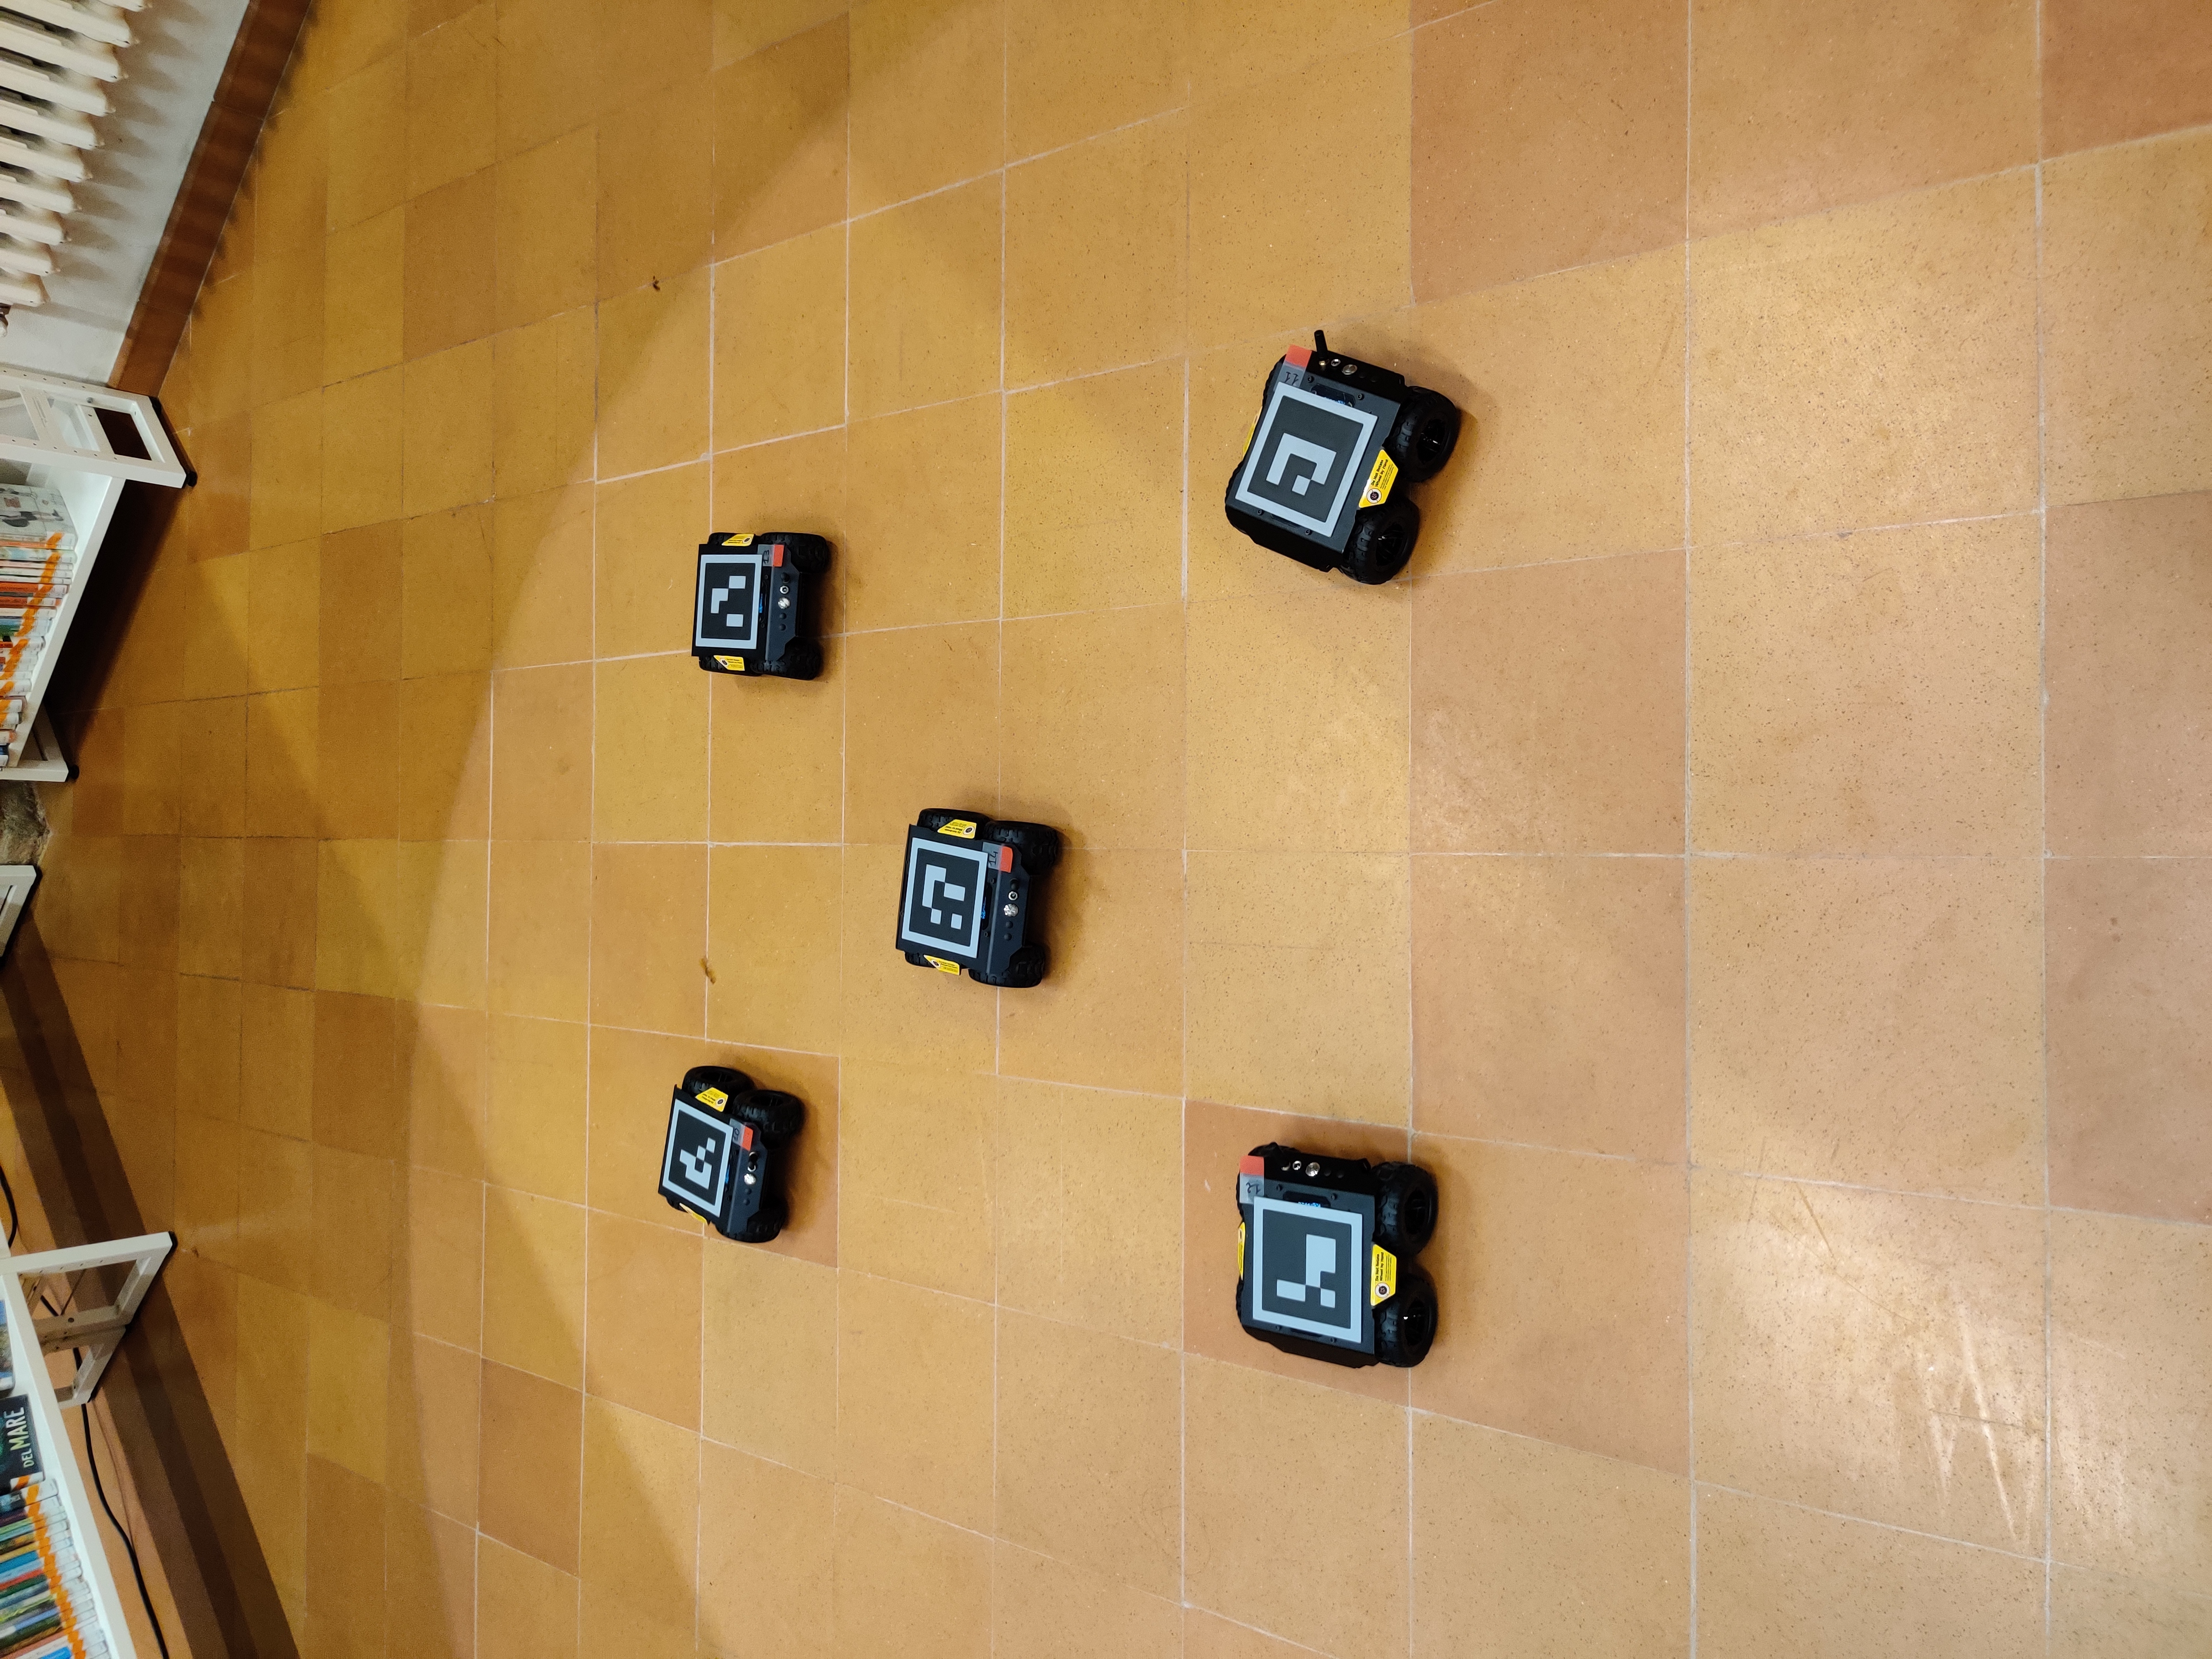
\includegraphics[width=0.8\linewidth, angle=-90]{./figures/Valutazione/robot.jpg}
	\caption{Robot identificati da marker ArUco}
	\label{fig:robot}
\end{figure}

\begin{figure}[h!]
	\centering
	\includegraphics[width=0.6\linewidth]{./figures/Valutazione/robot1.jpg}
	\caption{Sistema completo}
	\label{fig:system}
\end{figure}

\section{Sviluppi futuri}
Qui di seguito sono proposti alcuni possibili sviluppi futuri:
\begin{itemize}
	\item miglioramento hardware (calcolatore e fotocamera) per rendere il sistema più rapido e preciso;
	\item aggiunta di più camere per ampliare il campo visivo e garantire una stima della profondità più accurata;
	\item utilizzo di sistemi alternativi per calibrare la camera come ChArUco boards, così da permettere calibrazioni precise e allo stesso tempo flessibili in caso di occlusioni.
\end{itemize}

%----------------------------------------------------------------------------------------
% BIBLIOGRAPHY
%----------------------------------------------------------------------------------------

\backmatter
\printbibliography

\chapter*{Ringraziamenti}
Al termine di questa tesi mi sembra doveroso ringraziare tutte le persone che mi hanno aiutato a raggiungere questo obiettivo.

In primis ci tengo a ringraziare il Prof. Mirko Viroli, sempre disponibile e professionale, grazie al quale ho avuto la possibilità di prendere parte ad un progetto interessante e innovativo, che mi ha permesso di espandere le mie conoscenze e consolidare le competenze acquisite durante questi tre anni.
Un ringraziamento speciale va al Dott. Gianluca Aguzzi che mi ha seguito durante tutta la stesura della tesi, fornendomi sempre un aiuto ove necessario in maniera pronta e gentile.

Non posso non ringraziare tutta la mia famiglia, in particolare i miei genitori e mio fratello, che in questi anni hanno sempre saputo comprendermi e anche quando le mie ansie prendevano il sopravvento erano sempre pronti ad ascoltarmi e rassicurarmi. 

Grazie ai miei genitori per aver supportato ogni mia decisione e per avermi reso quello che sono, grazie a mio fratello con cui so di potermi sempre confidare, grazie ai miei nonni per essere fonte di ispirazione e per credere sempre in me. 

Un ringraziamento speciale va ai miei amici più stretti, quelli con cui sono cresciuto e quelli che ho avuto la fortuna di conoscere più avanti, con i quali ho affrontato mille avventure e grazie ai quali riesco sempre ad essere me stesso e a dimenticarmi delle mie preoccupazioni.

Un grazie ai miei colleghi dell'università con cui ho condiviso gioie e dolori di questo percorso universitario, dai pranzi assieme sino ai progetti d'esame più difficili. Vi ringrazio di aver reso le mie giornate in università meno impegnative e di avermi sempre aiutato in situazioni di difficoltà.

\end{document}
